% !TeX options = -shell-escape
\documentclass[11pt]{article}

\usepackage[utf8]{inputenc}
\usepackage[T1]{fontenc}
\usepackage[margin=2.5cm]{geometry}
\usepackage[english, magyar]{babel}
\usepackage{amsmath}
\usepackage[pdftex,unicode,raiselinks,colorlinks=true]{hyperref}
\hypersetup{
    colorlinks=true,
    linkcolor=black,
    citecolor=black,
    filecolor=black,
    urlcolor=black,
    menucolor=black
}
\usepackage{enumitem}
\usepackage{multicol}
\usepackage{setspace}
\usepackage{subcaption}
\usepackage{caption}
\DeclareCaptionLabelFormat{hungarianfigure}{#2.~ábra}
\captionsetup[figure]{
    labelformat=hungarianfigure,
    labelsep=period
}
\usepackage{float}
\usepackage[autostyle=true]{csquotes}
\usepackage[nameinlink,noabbrev]{cleveref}
\usepackage[backend=biber,style=ieee,sorting=none]{biblatex}
\usepackage{graphicx}
\usepackage{minted}
\usepackage{tikz}
\usepackage{wrapfig}
\usetikzlibrary{positioning, arrows.meta}


\addbibresource{hivatkozasok.bib}

\onehalfspacing

\hyphenation{pre-sence vi-su-alized si-mu-la-tions mo-le-cu-lar se-ve-ral cha-rac-te-ris-tic CoNSEnsX}

\begin{document}

    \hypersetup{pageanchor=false}
    \begin{titlepage}
        \centering

        {\Huge\bfseries
        Mozgásszervi rehabilitációt támogató, szenzoradatokat feldolgozó keresztplatformos alkalmazás fejlesztése
        \par}

        \vspace{1.2cm}

        {\Large Önálló laboratórium dokumentáció\par}

        \vspace{2cm}


        
\includegraphics[width=0.42\textwidth]{itk_logo_eng.png}

        \vspace{2cm}

        \begin{minipage}{0.65\textwidth}
            \large
            \begin{tabular}{ll}
                Készítette: & Győrfi Bernadett (DNKZ89)\\
                Témavezető: & Dr.Grand László \\
                Szak: & Molekuláris Bionika Mérnök\\
                Tantárgy: & Önálló laboratórium \\
            \end{tabular}
        \end{minipage}

        \vfill

        {\large
        Pázmány Péter Katolikus Egyetem\\
        Információs Technológiai és Bionikai Kar\\
        Budapest, Magyarország\\
        2026
        \par}

    \end{titlepage}

    \hypersetup{pageanchor=true}


    \renewcommand{\contentsname}{Tartalomjegyzék}
    \tableofcontents

    \newpage
    \section{Feladat leírása}

A projekt célja egy Parkinson-kóros betegek rehabilitációját támogató mobilalkalmazás fejlesztése volt.
A betegségre jellemző motoros tünetek (például a testtartási instabilitás vagy a járászavarok) miatt a
fizikai rehabilitáció kiemelt fontosságú.
Az alkalmazás célja ennek megfelelően nem orvosi diagnózis felállítása, hanem a rehabilitációs
folyamat informatikai támogatása és a gyakorlatok során keletkező adatok strukturált kezelése.

A megoldás a Sensoria által kifejlesztett viselhető szenzor (okoszokni) adatait dolgozza fel.
A szenzor a gyakorlatok közben valós időben szolgáltat információt a sarok, a lábfej és a
lábujjak terheléséről, valamint a láb x, y és z irányú gyorsulásáról, a zokni összeállítása
az \ref{fig:sock}. ábrán látható.

\begin{wrapfigure}{r}{0.4\textwidth}
    \centering
    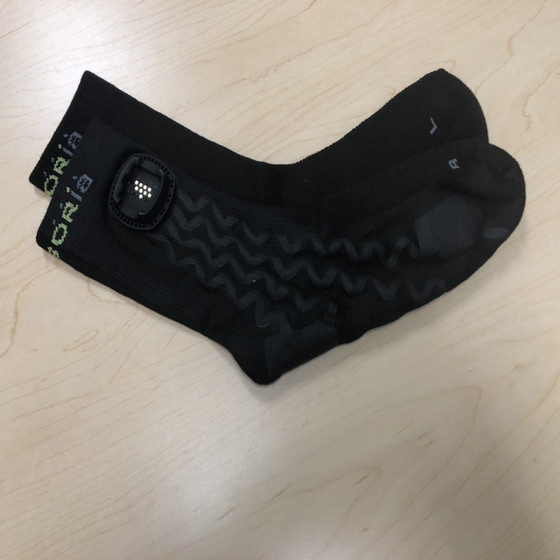
\includegraphics[width=0.4\textwidth]{images/sock}
    \caption{A Sensoria okoszokni \cite{sensoria2016walk}, látható a bluetooth csatlakozó
    helye a zokni szárán és a talp részén a szenzorok elhelyezkedése.}
    \label{fig:sock}
\end{wrapfigure}

Ezeket az adatokat az alkalmazás fogadja, feldolgozza, majd az adott munkamenethez kapcsolva
tárolja. A mérési folyamatot videós útmutató is kiegészíti, amely lehetőséget ad a
gyakorlatok megtekintésére és megfelelő végrehajtására.


A tervezett rendszernek több fő funkciót kellett megvalósítania.
Ezek közé tartozott az előre rögzített gyakorlatok listázása és kiválasztása,
a mérési munkamenet indítása és lezárása, a Sensoria okoszokniból érkező szenzoradatok kezelése,
a videós komponensek integrálása, valamint az eredmények áttekinthető megjelenítése.
Fontos szempont volt az is, hogy a korábban rögzített munkamenetek később visszakereshetők
és megtekinthetők legyenek.


A fejlesztés során az egyik tervezési szempont volt a moduláris felépítés.
Ennek köszönhetően az alkalmazás később új rehabilitációs feladatokkal,
további mérési módszerekkel vagy új elemzési funkciókkal is bővíthető maradhat.



















    \section{Bevezetés}

A Parkinson-kór a központi idegrendszer progresszív megbetegedése, amely elsősorban a
mozgásszabályozást érinti. A betegség gyakori motoros tünetei közé tartozik a remegés,
az izommerevség, a mozgáslassulás (bradykinesia), valamint az egyensúly és a koordináció romlása. \cite{author2025physiotherapy}
Ezek a tünetek a betegség előrehaladtával egyre nagyobb mértékben befolyásolhatják a
beteg járását, testtartását, mindennapi aktivitását és önállóságát.

A gyógyszeres kezelés mellett fontos szerepet kap a mozgásterápia és a fizioterápia,
amelyek célja a mozgásfunkciók fenntartása, a járás és az egyensúly javítása, valamint az
életminőség támogatása.\cite{osborne2022physical} rehabilitáció általában hosszabb távú folyamat,
amelynek eredményességét jelentősen befolyásolhatja a gyakorlatok rendszeressége
és helyes végrehajtása.


A terápiás alkalmakon kívül végzett gyakorlatok esetében kihívást jelenthet a végrehajtás
követése és értékelése. A szakember számára gyakran korlátozott mennyiségű információ áll
rendelkezésre arról, hogy a beteg a gyakorlatokat milyen módon és milyen minőségben végezte el.
Emiatt a rehabilitációban egyre fontosabbá válnak azok a digitális megoldások,
amelyek a gyakorlatokhoz kapcsolódó adatokat mérhető és később is elemezhető formában rögzítik.
\cite{rossi2022parkinson}


A mobilalkalmazások és távrehabilitációs rendszerek lehetőséget adnak arra, hogy a beteg a
terápiás alkalmakon kívül is irányított formában végezzen feladatokat.
Egy ilyen funkciókat ellátó alkalmazás nemcsak a feladatok megjelenítésében segíthet,
hanem a mérési folyamat egységesítésében és az adatok rendszerezésében is.
Ez különösen olyan esetekben hasznos, amikor a hosszabb távú követés vagy a
gyakorlatok összehasonlíthatósága fontos szempont. \cite{chen2024application}


A digitális rehabilitáció egyik lényeges eleme az objektív mérési adatok gyűjtése.
A viselhető szenzorok előnye, hogy a mozgás közben, a felhasználót viszonylag kevéssé
zavarva képesek adatokat szolgáltatni. \cite{paci2020design} Parkinson-kór esetén különösen hasznosak lehetnek azok
a szenzorok, amelyek a járáshoz, egyensúlyhoz vagy testsúlyáthelyezéshez kapcsolódó információkat
mérik. A lábon viselt eszközök ebből a szempontból kiemelt jelentőségűek, mivel közvetlenül a
talajkontaktusról, a terhelési mintázatról és a láb mozgásáról adhatnak információt.


A Sensoria okoszokni ilyen típusú viselhető mérőeszköz, amely a talp különböző részein
jelentkező nyomásviszonyokról és a láb mozgásáról szolgáltat adatokat. \cite{sensoria2016walk}
Ez a mérési megoldás jól illeszkedik egy mobilalkalmazással támogatott rehabilitációs rendszerhez,
mivel nem igényel nagyméretű, helyhez kötött laboratóriumi eszközöket.
Az így gyűjtött adatok alapot adhatnak a gyakorlatok későbbi áttekintéséhez, összehasonlításához
és további elemzéséhez.


A jelen dolgozat egy ilyen, Sensoria okoszoknival együttműködő mobilalkalmazás fejlesztését
mutatja be. A következő fejezetekben az alkalmazás felépítése, fő komponensei, az adatrögzítés
folyamata, valamint az eredmények megjelenítésének módja kerül ismertetésre.

















    \section{A konkrét munkafolyamat ismertetése}
    \subsection{Az alkalmazás áttekintése}

A fejlesztett alkalmazás elsősorban Android operációs rendszerre készült. 
A projekt alapját a Kotlin Multiplatform adja, amely lehetővé teszi, hogy az alkalmazás üzleti 
logikájának és adatkezelésének egy része platformfüggetlen módon készüljön el \cite{kotlinmultiplatform}.
Ennek előnye, hogy a közös kódrészek a későbbiekben más platformokon, például Androidon és iOS-en is
felhasználhatók. Az iOS-verzió tényleges implementálása és tesztelése azonban teszteszköz hiányában
ezen projekt során nem történt meg, ezért a dolgozat elsősorban az Androidos megvalósításra fókuszál.

A fejlesztés nyelve Kotlin volt, amely az Android-fejlesztésben széles körben támogatott, modern 
programozási nyelv. A Java nyelvvel való együttműködése miatt jól illeszkedik az Android környezetbe,
ugyanakkor számos olyan nyelvi funkciót kínál, amely megkönnyíti a biztonságosabb és átláthatóbb kód 
írását, például a tömörebb szintaxis és az adatosztályok használata. \cite{kotlinandroid}

A felhasználói felület (UI) a Jetpack Compose keretrendszer komponenseiből épül fel. A hagyományos,
imperatív (XML-alapú) Androidos nézetekkel szemben a Compose deklaratív megközelítést alkalmaz: az egyes
képernyők (Composable függvények) automatikusan és dinamikusan újrarajzolják magukat (recomposition),
amint az alkalmazás mögöttes állapota megváltozik \cite{compose}.


\subsubsection{A rendszer felépítése és folyamata}

A rendszer felépítése több, egymástól elkülönített komponensből áll :
\begin{itemize}
    \item A felhasználói felületet megvalósító képernyők 
    \item A munkamenet állapotát kezelő logika 
    \item A szenzoradatok fogadásáért és feldolgozásáért felelős részek 
    \item Adattárolási és visszakeresési mechanizmusok 
    \item Eredmények megjelenítésére szolgáló komponensek 
\end{itemize}

Ezek a komponensek együttműködve alkotják meg a teljes alkalmazást, és a következő felhasználói
folyamatot valósítják meg :
\begin{enumerate}
    \item Az alkalmazás indítása, mely során a főképernyő jelenik meg.
    \item A Sensoria eszköz csatlakoztatása Bluetooth Low Energy (BLE) protokollon keresztül,
    és a nyers szenzoradatok fogadása.
    \item A gyakorlatok listájának megjelenítése, amely lehet előre meghatározott vagy a
    felhasználó által kiválasztott gyakorlatokat tartalmazhat.
    \item A mérés indítása.
    \item A szenzoradatok valós idejű fogadása, illetve a gyakorlatok végrehajtásának videós megjelenítése.
    \item A mérés lezárása, amely során a gyakorlatokhoz kapcsolódó adatok mentése történik.
    \item A mérés eredményeinek megjelenítése, amely lehetőséget ad a gyakorlatok áttekintésére és összehasonlítására.
    \item A korábban rögzített munkamenetek visszakeresése és megtekintése.
\end{enumerate}

A dokumentáció a további fejezetekben ezeknek a komponenseknek a részletes ismertetésére,
valamint a fejlesztés során felmerülő kihívásokra és megoldásokra fókuszál.
    \subsection{Alkalmazásarchitektúra}

Az alkalmazás felépítése több, egymástól jól elkülöníthető komponensből áll,
Ez a felépítés lehetővé teszi, hogy a felhasználói felület, állapotkezelés,
adatkezelés, adattároslás és a platformfüggő fukciók ne keveredjenek és az egyes
részek külön tesztelhetők és később könnyen bővíthetők legyenek.

\subsubsection{Legfelső réteg: Felhasználói felület}

Az alkalmazás lefelső rétegét a felhasználói felület (UI) alkotja. Ide tartoznak azok a képernők,
amelyekkel a felhasználó közvetlenül interakcióba lép. Az \code{App.kt} felel az alkalmazás
fő szerkezetéért és a képenyők közti navigációért. . A \code{ConfigScreen.kt} a mérés
előkészítéséhez kapcsolódó nézeteket tartalmazza, például a rehabilitációs feladatok kiválasztását.
Az \code{ExecutionScreen.kt} a munkamenet közbeni felületet valósítja meg, ahol a mérés vezérlése
és az aktuális gyakorlat követése történik. A \code{ResultsScreen.kt} az elkészült mérés
eredményeit jeleníti meg, míg a \code{SavedSessionScreen.kt} a korábban rögzített munkamenetek
kezeléséhez kapcsolódik. Ezek a képernyők nem önállóan végzik az adatfeldolgozást,
hanem az alkalmazás állapotkezelő és adatkezelő rétegeivel kommunikálnak.

\subsubsection{UI és háttérlogika közötti kapcsolat}

A felhasználói felület és a háttérlogika közötti kapcsolatot a \code{SessionViewModel.kt}
biztosítja. A ViewModel szerepe, hogy összefogja a munkamenet aktuális állapotát, és közvetítő
rétegként működjön a képernyők, az adattárolás, a szenzorkezelés és az elemző modulok között.
Ennek köszönhetően a képernyőknek nem kell közvetlenül ismerniük például a fájlkezelés vagy
a Bluetooth-kommunikáció részleteit.
A ViewModel kezeli, hogy a mérés milyen állapotban van, milyen adatok érkeztek be, mikor kell 
menteni az eredményeket, illetve mikor kell frissíteni a felhasználói felületen megjelenő
információkat.

\subsubsection{Adaszerkezet}

Az alkalmazás adatszerkezete külön objektumokkal van reprezentálva. A \code{SessionInfo.kt} a
munkamenethez kapcsololódó adatokat tartalmazza: a mérés azosításához és visszakereséséhez
szükséges adatokat. Az \code{ExportedTasks.kt} az adott feladatait írja le, benne van a feladat
neve és végrehajtási ideje. Az \code{ExportedSensorData} az adott nyomás és gyorsulás értékeket
gyűjti feladatoként és időlépésenként. Illetve a \code{SessionExport} rakja ezeket egybe,
tartalmazza az adott munkafolyamat információit és a gyűjtött szenzoradatokat. A
\code{SensoriaData} pedig a zokniból származó feldolgozott mérési adatokat írja le.
A \code{FullSessionResults.kt} és az \code{AnalysisModel.kt} az elemzés után létrejövő
eredmények és összesített mutatók tárolására szolgálnak. Mivel a tesztek során nem mindig
állt rendelkezésre a zokni, illetve nem volt szükség a Bluetooth kapcsolatra az adott funkciók
írásához és teszteléshez, ezért egy "hamis adat generátor" is implementálva lett az alkalmazás
írása közben ezt a logikát tartalmazza a \code{SensoriaData.kt}, a valósághoz valamennyire
közel álló szenzoradatokat hoz létre, amelyekkel a többi folyamat működése vizsgálható.
Az adatmodellek célja, hogy az alkalmazás különböző részei ugyanazokat az információkat egységes,
jól definiált formában használják.

\subsubsection{Adattárolás}

Ezen réteg feladata a mentés, betöltés és exportálás. A \code{FileStorage.kt} felelős a fájlok
létrehozásáért, olvasásáért és írásáért, amelyet a \code{SessionViewModel.kt} irányít.

\subsubsection{Szenzoros réteg}

A réteg a Sensoria okoszoknival történő kommunikációt és az onnan érkező adatok értelmezését
valósítja meg. A \code{SensoriaBluetoothManager.kt} kezeli a Bluetooth-kapcsolatot, vagyis az
eszközhöz való csatlakozást és az adatcsomagok fogadását. A beérkező nyers adatok önmagukban még
nem használhatók közvetlenül az alkalmazás többi része számára, mert hexadecimális kódként érkeznek
ezért szükség van dekódolásra. Ezt a feladatot a \code{SensoriaDecoder.kt} végzi, amely a nyers
bájtokból értelmezhető mérési értékeket állít elő. A \code{BitReader.kt} az alacsonyabb szintű
bit- és bájtolvasási műveleteket segíti, amelyek a szenzoradatok pontos feldolgozásához szükségesek. A feldolgozott értékek végül a SensoriaData.kt adatmodellben jelennek meg, így a rendszer többi része már strukturált formában tud velük dolgozni.

\subsubsection{Kamera és videó}

Ezek a funkciók szintén külön vannak kezelve. A \code{CameraPreview.kt} a mérés közbeni
kameraelőnézet megjelenítéséért felel, ezzel a felhasználó láthatja a saját mozgását a
feladat végzése közben. A \code{VideoPlayer.kt} a gyakorlatok videós megjelenítésért felelős.
Mivel ezek az osztályok operációsrendszer-specifikusak, ezért meg vannak írva Android-specifikusan is.

\subsubsection{Adatelemzés}

Az elemzési réteg a rögzített adatokból számított eredmények előállításáért felel.
A \code{SessionAnalyzer.kt} a munkamenet egészének kiértékelését végzi, vagyis a rendelkezésre
álló szenzoradatokból és feladatadatokból állít elő összesített eredményeket.
A \code{StabilityCalculator.kt} speciálisabb számításokat tartalmaz, amelyek a
stabilitással kapcsolatos mutatók meghatározására szolgálnak.
Ezek az eredmények nem diagnosztikai következtetések, hanem a munkamenet későbbi
áttekintését és összehasonlítását segítő információk.





    \newpage
    \section{Felhasználói felület}

A felhasználói felület nem egyetlen összetett nézetben tartalmazza az alkalmazás összes funkcióját,
hanem a munkamenet fő lépéseihez igazodva külön képernyőkre bontja azokat.
Ez a felépítés segíti az áttekinthetőséget, mivel a felhasználó minden lépésben csak az adott
művelethez szükséges információkkal és vezérlőelemekkel találkozik.


\subsection{Konfigurációs képernyő}

A konfigurációs képernyő a munkamenet előkészítésére szolgál. Itt hozható létre a
Bluetooth-kapcsolat a Sensoria okoszoknival, amelynek állapotáról az alkalmazás visszajelzést
ad a felhasználónak. A sikeres csatlakozás után a felhasználó megadhatja a nevét,
amely a későbbiekben a mérés azonosítására szolgál.


A rehabilitációs mozgássorozat kétféleképpen állítható össze:
\begin{itemize}
    \item Egy előre meghatározott gyakorlatsor használata, amely egy specifikusan
    összeállított rehabilitációs feladatsort tartalmaz. Ebben az esetben a gyakorlatok sorrendje
    adott, a hozzájuk tartozó időtartamok azonban módosíthatók.
    \item Egyéni feladatsor összeállítása. Ez akkor hasznos, ha az előre definiált gyakorlatsor
    nem illeszkedik a felhasználó aktuális rehabilitációs szakaszához vagy állapotához.
    Ilyenkor a felhasználó egy legördülő listából választhatja ki a kívánt gyakorlatokat,
    megadhatja azok időtartamát, majd tetszőleges sorrendben hozzáadhatja őket a munkamenethez.
\end{itemize}


A konfigurációs képernyőről indítható el a mérés, valamint innen érhetők el a
korábban mentett munkamenetek is. A képernyő így a mérési folyamat kiindulópontjaként működik.


\subsection{Végrehajtási képernyő}

A végrehajtási képernyő a konfigurációs képernyőről indított mérés után jelenik meg.
A mérés megkezdése előtt a felhasználó egy felugró ablakban (dialog) választhatja ki a
kívánt vizuális visszacsatolási módot.
Lehetőség van csak a feladatot bemutató videó megjelenítésére,
csak az előlapi kamera képének megjelenítésére, illetve a kettő egyidejű,
egymás melletti megjelenítésére.


Minden gyakorlat előtt egy rövid, öt másodperces előkészítő szakasz jelenik meg.
Ebben az időszakban a felhasználó a gyakorlatot bemutató videót látja,
így még a mérés kezdete előtt megfigyelheti a helyes végrehajtást.
A tényleges adatgyűjtés és a gyakorlat végrehajtása csak ezt követően indul el.


A mérés a munkamenet közben bármikor megszakítható. Ebben az esetben az alkalmazás nem menti el
a munkamenetet, így nem keletkezik hiányos vagy félbeszakított adatokon alapuló elemzés.
Ez fontos szempont az eredmények értelmezhetősége és a tárolt adatok következetessége miatt.


A gyakorlatok végrehajtása közben a felület a kiválasztott megjelenítési módnak megfelelő
videós tartalmat jeleníti meg. A videó alatt a statikus szöveges instrukciók szerepelnek,
illetve a stabilitási adatok jelennek meg, amelyek az aktuális végrehajtásról adnak közvetlen
visszajelzést a felhasználónak.


\subsection{Eredményképernyő}

A mérés lezárása után az alkalmazás automatikusan az eredményképernyőre navigál.
Ez a felület a munkamenethez tartozó összesített információkat jeleníti meg strukturált formában.
A cél az, hogy a rögzített adatok ne nyers szenzorértékekként jelenjenek meg, hanem olyan
áttekinthető formában, amely segíti a mérés értelmezését.


Az eredményképernyőn megjelennek a munkamenet azonosításához szükséges alapadatok,
például a felhasználó neve és a mérés időpontja.
Emellett láthatók a végrehajtott gyakorlatokhoz kapcsolódó eredmények,
valamint a szenzoradatokból számított mutatók. Ezek az információk a munkamenet későbbi
áttekintését és összehasonlítását támogatják.

\subsection{Mentett munkamenet képernyő}

A mentett munkamenetek képernyője a korábban rögzített mérések elérésére szolgál.
A felület listában jeleníti meg az elmentett munkameneteket, amelyek közül a felhasználó
kiválaszthatja a megtekinteni kívánt elemet. A kiválasztott munkamenet betöltése után az
alkalmazás megjeleníti az ahhoz tartozó eredményképernyőt.


A listázás során  az egyes mérések egyértelműen azonosíthatók a felhasználó neve és a
méréshez tartozó időbélyeg segítségével.
Így több eltárolt munkamenet esetén is visszakereshető, hogy melyik mérés kihez és mikorhoz
kapcsolódik.


A nem kívánt vagy már nem szükséges munkamenetek manuálisan törölhetők a telefon tárhelyéről.
Ez lehetőséget ad arra, hogy a felhasználó vagy a fejlesztő szükség esetén eltávolítsa a már nem
releváns mérési adatokat.


    \section{A Sensoria okoszokni integrációja}

Az alkalmazás egyik központi eleme a Sensoria okoszokniból érkező szenzoradatok kezelése. A
zokni külső mérőeszközként kapcsolódik az alkalmazáshoz, és a gyakorlatok végrehajtása közben
folyamatosan küldi az adatokat. A feladat ezért nemcsak az adatok fogadása volt, hanem azok
értelmezése és olyan formába alakítása is, amely az alkalmazás további részei számára már
feldolgozható.

A kommunikáció Bluetooth Low Energy-kapcsolaton keresztül történik. A kapcsolat kezeléséért egy külön
komponens felel, amely az okoszoknihoz való csatlakozást, a kapcsolat állapotának figyelését és az
adatcsomagok fogadását végzi. Ez azért különösen fontos, mert a Bluetooth-kommunikáció platformfüggő
és állapotérzékeny folyamat: kezelni kell a csatlakozás létrejöttét, az esetleges kapcsolatvesztést,
valamint azt is, hogy az adatok csak sikeres kapcsolat esetén kerüljenek feldolgozásra.

Az alkalmazás egy \code{ScanFilter} segítségével a Sensoria szolgáltatáshoz tartozó UUID alapján szűri
az elérhető eszközöket. Emellett az eszköz neve alapján is ellenőrzi, hogy valóban a zokniról van-e szó.
Amikor megtalálja a megfelelő eszközt, leállítja a keresést, majd \code{connectGatt} hívással GATT-
kapcsolatot hoz létre a zoknival. A GATT, vagyis a Generic Attribute Profile, a Bluetooth Low Energy
eszközök közötti adatkommunikáció egyik alapvető modellje. Ebben a felépítésben az okoszokni
szerverként működik, amely különböző szolgáltatásokat és azokon belül characteristic-eket tesz
elérhetővé. Az alkalmazás kliensként kapcsolódik ehhez a szerverhez, majd a megfelelő szolgáltatáson
keresztül fogadja a mérési adatokat.

A kapcsolat felépítése után indul a BLE service discovery folyamat. Ennek során az alkalmazás
megkeresi a Sensoria szolgáltatáshoz tartozó service UUID-t, majd azon belül kiválasztja azt a
characteristic-et, amely támogatja a \code{NOTIFY} vagy \code{INDICATE} tulajdonságokat. A
characteristic-ek a BLE szolgáltatáson belüli adattároló vagy adatküldő pontokként értelmezhetők.
A \code{NOTIFY} azt jelenti, hogy az eszköz új adat érkezésekor automatikusan értesítést küld a
kliensnek, visszaigazolás nélkül. Az \code{INDICATE} ehhez hasonlóan működik, de a kliens oldaláról
visszaigazolást is igényel. Erre azért van szükség, mert a szenzoradatok nem egyszeri lekérdezéssel
érkeznek, hanem a zokni folyamatosan küldi őket a mérés során.

Az értesítések fogadásához az alkalmazás engedélyezi a kiválasztott characteristic notification
funkcióját. Ehhez a Client Characteristic Configuration Descriptor, röviden CCCD, beállítása szükséges.
Ez azt határozza meg, hogy a kliens kér-e értesítéseket vagy indikációkat az adott characteristic
változásairól. A beállítás után a zokni képes folyamatosan továbbítani az új
szenzoradatokat az alkalmazás felé.

A beérkező adatok kezelése callback-alapúan történik. Amikor a zokni új adatcsomagot küld,
az Android rendszer meghívja az \code{onCharacteristicChanged} függvényt. A megvalósítás figyelembe
veszi, hogy Android 13-tól megváltozott ennek a függvénynek a szignatúrája, ezért a kódban a régebbi
és az újabb API-verzióhoz tartozó változat is szerepel. Mindkét esetben a beérkező bájttömb kerül
továbbításra a csomagfeldolgozó logikának.

A szenzoradatok továbbítása az alkalmazás többi része felé Kotlin Flow segítségével valósul meg.
A \code{connectAndListen} függvény egy \code{Flow<SensoriaData>} típust ad vissza, amelybe a beérkező
és sikeresen dekódolt mérési adatok kerülnek. A callback-alapú Android BLE működés és a
coroutine-alapú alkalmazáslogika összekapcsolására a megvalósítás \code{callbackFlow}-t használ.
Ez lehetővé teszi, hogy a Bluetooth callbackekből érkező események reaktív adatfolyamként
jelenjenek meg az alkalmazás többi komponense számára. A kapcsolat lezárásakor az \code{awaitClose}
blokk gondoskodik a scan leállításáról, a GATT-kapcsolat bontásáról és az erőforrások felszabadításáról.

A nyers adatcsomagok dekódolását külön logika végzi. A Sensoria okoszokniból érkező bájtok nem
közvetlenül értelmezhetőek, ezért az alkalmazás bitenként olvassa ki belőlük a szükséges mezőket.
Ehhez a \code{BitReader} segédosztályt használja, amely egy bájttömbből megadott számú bitet tud
sorban kiolvasni. A dekódolás során az alkalmazás először átugorja a csomag fejlécéhez és metaadataihoz
tartozó mezőket, például az üzenettípust, a kontextust és az időzítési mezőket, majd kiolvassa a mérés
szempontjából fontos értékeket.

A feldolgozás során három nyomáscsatorna és három gyorsulási komponens kerül kinyerésre.
A \code{ch0}, \code{ch1} és \code{ch2} mezők a talp különböző pontjain mért nyomásértékeket
reprezentálják, míg az \code{accelX}, \code{accelY} és \code{accelZ} a láb három tengely menti
gyorsulását tartalmazzák. A csomagban található magnetométer-adatokat az alkalmazás jelenlegi
verziója kiolvassa, de nem használja fel az eredményképzéshez. A dekódolás eredménye egy
\code{SensoriaData} objektum, amely már strukturált formában tartalmazza a további feldolgozáshoz
szükséges adatokat.

A \code{SensoriaData} adatmodell a szenzorból származó mérési értékek mellett időbélyeget is tartalmaz.
Ez azért fontos, mert a szenzoradatok sorrendje és időbeli elhelyezkedése a későbbi feldolgozás során
is lényeges. Az adatmodellben szerepel a feladathoz tartozó információ is, így az egyes mérési pontok
összekapcsolhatók azzal a gyakorlattal, amelynek végrehajtása közben keletkeztek.

A szenzoradatok az aktuális munkamenethez kapcsolódva kerülnek eltárolásra.
A mérés indításakor az alkalmazás elkezdi gyűjteni a \code{Flow}-ból érkező \code{SensoriaData}
objektumokat, majd ezeket a feladatokhoz és a munkamenethez rendeli.
A mérés lezárásakor az összegyűjtött adatok a többi munkamenet-információval együtt mentésre kerülnek.
Így egy korábbi mérés visszatöltésekor nemcsak a munkamenet alapadatai, hanem a hozzá tartozó
szenzoros mérési adatok is elérhetők.

A megvalósítás során az Android Bluetooth-jogosultságok kezelésére is figyelni kellett. Újabb Android-
verziókon a Bluetooth-eszközök kereséséhez és a kapcsolódáshoz külön engedélyek szükségesek, például
a \code{BLUETOOTH\_SCAN} és a \code{BLUETOOTH\_CONNECT}. Régebbi verziókon a BLE scan működéséhez
helymeghatározási jogosultságra is szükség lehet. Az alkalmazás ezért a Bluetooth-műveletek indítása
előtt ellenőrzi, hogy a szükséges rendszerengedélyek rendelkezésre állnak-e.

    \section{Kamera és videókezelés}

Az alkalmazás szenzoradatok mellett videós tartalom is megjelenik. A videós funkciók a végrehajtási
képernyőhöz kapcsolódnak. A munkamenet elején a felhasználó kiválaszthatja,
hogy milyen nézetet szeretne használni: csak a bemutatóvideót, csak az előlapi kamera képét,
vagy a kettőt egyszerre, egymás mellett. Ez rugalmasabb használatot tesz lehetővé, mert a felhasználó
eldöntheti, hogy inkább a minta alapján szeretné követni a gyakorlatot,
vagy a saját mozgását szeretné látni végrehajtás közben.

A bemutatóvideó minden feladat előtt rövid előkészítő szakaszban jelenik meg.
Ez alatt a felhasználó még nem végez mérést, hanem megfigyelheti, hogyan kell a következő
gyakorlatot végrehajtani. A tényleges adatgyűjtés csak az előkészítő szakasz után indul el,
így a rögzített szenzoradatok már a gyakorlat végrehajtásához kapcsolódnak. A kamera-előnézet
célja nem önálló videóelemzés, hanem a mozgás felhasználó általi vizuális követésének támogatása.


A videók kezelése részben platformfüggő feladat, ezért az alkalmazásban különválik a közös felület
és az Android-specifikus megvalósítás. A közös kódrészben a videólejátszáshoz tartozó absztrakció
szerepel, míg az Androidhoz kötődő működés külön implementációban kap helyet.





    \section{Adattárolás és exportálás}

Az alkalmazásban az adattárolás szigorúan a mérés lezárásához kapcsolódik. A munkamenet közben a
rendszer a szenzoradatokat a memóriában rakja. Ezek az adatsorok csak abban az esetben kerülnek
véglegesen mentésre, ha a felhasználó szabályosan végrehajtja és befejezi a mérést. Amennyiben a
munkamenet megszakításra kerül, az alkalmazás eldobja a memóriatartalmat,

\subsection{DTO tervezési minta és Szerializáció}

A mentés megkezdése előtt az alkalmazás összeállítja a teljes munkamenetet leíró adatszerkezetet.
Az alkalmazás belső, futásidejű állapotát
reprezentáló modellek (például az aktív \texttt{SensoriaData} objektumok) nem egyeznek meg azzal
a formátummal, amely hosszú távú tárolásra optimalizált.

A probléma feloldására a rendszer a Data Transfer Object (DTO) tervezési mintát alkalmaztam.
Az aktuális állapotból egy külön exportobjektum-hierarchia (\texttt{SessionExport}, \texttt{SessionInfo},
\texttt{ExportedSensorData}) épül fel. Így mentett munkamenet önmagában is, kontextusával együtt
(metaadatok, feladatok paraméterei, normalizált gyorsulás) értelmezhető legyen a későbbi feldolgozás során.

A memóriában lévő objektumok fájlba írását a \texttt{kotlinx.serialization} keretrendszer végzi,
amely platformfüggetlen módon alakítja át a Kotlin adatosztályokat olvasásra
alkalmas  JSON (JavaScript Object Notation) szöveges formátummá \cite{kotlinserialization}.

\subsection{Biztonságos fájlkezelés}

A generált JSON fájl tárolása az Android operációs rendszer belső, izolált tárhelyén
(\texttt{Context.filesDir}) történik \cite{androidstorage}. Az itt tárolt fájlokhoz más alkalmazások
vagy külső felhasználók nem férhetnek hozzá, és az alkalmazás eltávolításakor a rendszer
automatikusan megsemmisíti őket, megelőzve az érzékeny adatok (pl. páciens azonosítók, egészségügyi mutatók)
kiszivárgását.

A fájlnevek generálása egy szigorú mintát követ,
amely tartalmazza a felhasználó nevét(Patient ID) és a mérés pontos időbélyegét
(pl. \texttt{session\_PT-001\_20260523\_...json}). Ez az elnevezés biztosítja a mérések
egyértelmű azonosíthatóságát és a mentett adatok listázását a
felhasználói felületen.


    \section{Eredmények számítása és megjelenítése}

A bemeneti adatok feladatonként címkézett, idősoros mérési pontokból állnak,
amelyek tartalmazzák a talpi nyomáscsatornák (\texttt{ch0, ch1, ch2}) nyers értékeit,
a normalizált háromtengelyű gyorsulási adatokat, valamint a rendszer-időbélyeget.


\textbf{\subsection{Statikus feladatok jelfeldolgozása}}

A statikus gyakorlatok (pl. kétlábas állás, tandem állás) során az algoritmus
elsősorban az egyensúlyi helyzet és a stabilitás megtartását vizsgálja
\cite{posturalcontrol}.

\subsubsection{Súlypontvándorlás (Center of Pressure - CoP)}

A súlypont kilengését a talp elülső része (lábujjak és talppárna) és a sarok közötti,
illetve a lábfej jobb és bal oldala közötti nyomáskülönbségek alapján számítom.
A vertikális tengelyen az algoritmus megvizsgálja, hogy a statikus mérés során a
sarokterhelés átlagos aránya meghaladja-e a 65\%-ot a teljes talpnyomáshoz
viszonyítva. Mivel a Parkinson-kóros betegekre gyakran jellemző a súlypont akaratlan
hátrahelyeződése, így a hátraesés kockázata mérhető. A horizontális és vertikális
kilengések  varianciájának összeadásával egy stabilitási mutatót kapunk.

\subsubsection{Remegési index (Tremor)}

A nyugalmi remegés kimutatására az algoritmus a háromdimenziós gyorsulásvektorok
euklideszi normájának (hosszának) varianciáját számítja ki.
A rendszer a statikus gravitációs hatást az átlagos gyorsulás levonásával vonja ki jelből,
így az eredmény a láb mikro-rezgéseinek intenzitását reprezentálja.

\subsection{Dinamikus feladatok jelfeldolgozása}

A mozgást igénylő feladatoknál (például helyben járás, séta) a fókusz a lépésciklusokra
és a mozgáskivitelezés minőségére helyeződik \cite{gaitanalysis}.

\subsubsection{Lépésdetektálás és sarokleütés (Heel Strike)}

A lépéseket a függőleges (z-irányú) gyorsulási adatok lokális maximumainak keresésével
 detektálja az algoritmus, egy küszöbérték (550) alkalmazásával. A szenzorzajból
eredő hamis dupla detektálások elkerülése érdekében a rendszer egy 15 mintavételi
ciklusos holtidőt alkalmaz a lépések között. A lépés talajra érésének pillanatában a
talpi nyomáseloszlás arányaiból kiszámítható a sarok érkezésének módja.
Ez megmutatja, hogy a felhasználó a sarkán gördül-e, vagy a Parkinson-kórra
jellemző csoszogó járást mutatja, ahol az előtalp terhelése a jellemző.

\subsubsection{Fáradási index}

A fáradás méréséhez a rendszer a munkamenet adatsorát megfelezi, majd kiszámítja
az első és a második félidőben mért 3D gyorsulási vektorok átlagos energiáját (hosszát).
A két érték közötti százalékos amplitúdócsökkenés megmutatja, hogy a gyakorlat végére
mennyire esett vissza a végtagmozgás dinamikája.

\subsection{Lefagyás (Freezing of Gait) detektálása}

A Freezing of Gait (FoG) egy hirtelen, átmeneti epizód, amikor a beteg képtelen
a járás folytatására. Detektálására az algoritmus egy 50 mintavételi pontból álló,
folyamatosan csúszó időablakot alkalmaz az adatsoron \cite{fogdetection}.
A lefagyást két egyidejű feltétel teljesülése azonosítja: a horizontális gyorsulások
varianciája egy adott küszöbérték fölé ugrik (magas frekvenciájú lábremegés jelentkezik),
miközben a maximális és minimális nyomásértékek különbsége minimális marad
(a súlypont nem mozdul el, tehát nincs tényleges lépés).

\section{Eredmények vizualizációja}

A feldolgozott eredmények megjelenítése a Jetpack Compose rajzoló API-ja (\texttt{Canvas})
segítségével történik, egyedi, hardveresen gyorsított grafikonokon.

\begin{itemize}
\item Talpi nyomáseloszlás (Hőtérkép): A három nyomásszenzor átlagos
értékeit egy lábfejet formázó alakzaton jeleníti meg, ahol a színátmenetek
(zöldtől a pirosig)  jelzik a terhelés mértékét.
\item Egyensúlyi helyzet (CoP Scatter Plot): Egy céltáblát formázó szórásdiagram,
amely a nyomáskülönbségek alapján pontokként rajzolja ki a feladatok alatti horizontális
és vertikális súlypontvándorlást.
\item \textbf{Lépésciklusok (Ritmus-vonal):} A függőleges gyorsulás utolsó
100 mérési pontját egy vonaldiagram ábrázolja, amely vizuálisan megmutatja a
lépések ritmusát, egyenletességét vagy az esetleges aszimmetriát.
\end{itemize}

\textbf{\subsection{A vizualizáció és az elemzés célja}}

A vizualizáció célja nem egy diagnosztikai eszköz létrehozása volt, hanem inkább példákon
keresztül bemutatni, hogy a gyakorlatok során gyűjtött adatok hogyan értelmezhetők és milyen
információkat hordozhatnak.
    \section{Tesztelés és validáció}

Az alkalmazás tesztelése elsősorban funkcionális szempontból történt.
A tesztelési fázis célja annak ellenőrzése volt, hogy a felhasználói folyamatok
hibamentesen végigvihetők-e, valamint hogy a méréshez kapcsolódó adatok a várt
formátumban menthetők és tölthetők vissza.

\subsection{Fizikai és emulált tesztkörnyezet}

A tesztelés két fő környezetben zajlott. A fejlesztési fázis nagy részében az
Android Virtual Device (AVD) emulátorok használata tette lehetővé a gyors iterációt
\cite{androidemulator}. Ennek segítségével a felhasználói felület (UI) vizuális elemei,
a képernyőméretekhez való alkalmazkodás és a fájlkezelési funkciók anélkül
voltak tesztelhetők, hogy minden alkalommal fizikai teszteszközt kellett
volna csatlakoztatni.

A tesztelés megtörtén fizikai eszközön is. Erre azért volt szükség, hogy a
Bluetooth Low Energy (BLE) kapcsolat stabilitása, az operációs rendszer szintű
jogosultságkérések, a hardveres kameraelőnézet, valamint a valós idejű,
aszinkron szenzoradatok fogadása valós körülmények között is igazolható legyen.

\subsection{Adatgenerálás (Mocking)}

Mivel a zokni nem volt elérhető a tesztelés minden fázisában, ezért az alkalmazás egy
beépítettem egy tesztadat-generátort (\texttt{MockDataGenerator}) , amely képes a
fizikai szenzor adatáramlását szimulálni \cite{syntheticdata}.

A generátor nem csupán statikus értékeket állít elő, hanem a kiválasztott rehabilitációs
feladat (pl. helyben járás, tandem állás) típusához igazodó, matematikailag modellezett
jelsorozatokat generál:
\begin{itemize}
\item Dinamikus mozgás szimulálása:  Helyben járás esetén az algoritmus egy
belső időzítő alapján végigmegy a lépésciklus fázisain.
Különálló gyorsulás- és nyomásértékeket rendel a sarok földetéréséhez,
a talp gördüléséhez, az elrugaszkodáshoz és a lengési fázishoz.
\item Súlypontvándorlás: Statikus feladatoknál a generátor trigonometrikus függvények
(\texttt{sin}) segítségével szimulálja a test folyamatos, hullámszerű előre-hátra dőlését.
\item Zaj és patológiás tünetek: A valósághűség érdekében a rendszer random zajt generál
az adatokba a szenzorok 10-bites hardveres limitjein belül. Emellett dedikált logikát
tartalmaz a Parkinson-kórra jellemző mikro-remegések és ritka, véletlenszerű lefagyásos
(Freezing of Gait) epizódok szimulálására is.
\end{itemize}

A generált adatok használata lehetővé tette, hogy az adatgyűjtés folyamata, az UI
diagramok frissülése és az elemzési logika (pl. lépésdetektálás, varianciaszámítás)
folyamatosan tesztelhető maradjon. Mivel a szintetikus szenzoradatok felépítése
meghatározott, az adatfeldolgozó algoritmusok pontossága és helyessége a tesztelés
során ellenőrizhető volt.


    \section{Az alakalmazás további fejlesztési lehetőségei}

\subsection{Szerveres adattovábbítás és elemzés}

A jelenlegi alkalmazás a gyakorlat videóit és a  mérési adatokat a készüléken lokálisan tárolja, az
analízist a telefon saját erőforrásain végzi el és így jeleníti meg az adatokat.
Ez nagy mértékben korlátozza a számítás komplexitását és a gyakorlatok során gyűjtött adatok mennyiségét.
Erre lenne megoldás egy szerveres adattovábbítási és elemzési mechanizmus kialakítása, ez nem
csak a telefont tehermentesítené, de lehetővé tenné olyan matematikai adatelemzési módszerek
alkalmazását, amelyeket más környezet, például Python, R vagy MATLAB keretében könnyebben
lehet megvalósítani, mint Androidon.


\subsection{Platform kompatibilitás}

Ahogy a dolgozat elején is említésre került, a jelenlegi alkalmazás Android rendszerre van
megírva és tesztelve, mivel a Multiplatformos megközelítés lehetővé teszi, hogy később ez az
alkalmazás iOS-en is futtatható legyen, megfelelő teszt eszköz biztosításával az alkalmazás
iOS verziója is létrehozható a lokális környezetnek megfelelő videó- és fájlmenedzsment valamint
a Bluetooth-kapcsolat kezelésének megvalósításával.

\subsection{További adatelemzési módszerek}

A jelenlegi rendszerben az elemzés elsősorban egyszerű statisztikai mutatókra és ökényesen definiált
küszöbértékekre épül. Ezen módszerek szakemberrel való hitelesítése fontos lenne az
alkalmazás teszt verzióján való túllépéshez.

Illetve mivel a betegek testsúlya és mozgásmintázata eltérő, ezek a merev határértékek nem mindenkinél
egyformán pontosak. Egy idősoros adatokra felkészített neurális hálózat (pl. LSTM) vagy egy felügyelt
tanulással betanított modell (pl. Random Forest) képes lenne a nyers szenzoradatokból
automatikusan megtanulni az egyéni mintázatokat, ezáltal sokkal robusztusabbá téve a lépésdetektálást
és a Freezing of Gait (FoG) felismerését.

Gépi tanulás segítségével az alkalmazás képessé válhatna előrejelzések készítésére is,
például a jövőbeli esési kockázat megbecsülésére a járás asszimetriájának vagy a
stabilitás hosszú távú romlásának felismerésével. Implementálható lenne a teljes lépésciklus
folytonos fázisosztályozása (sarokleütés, gördülés, elrugaszkodás és lengési fázis
mikromásodperces elkülönítése).
    \section{Összegzés}

A feladat célja egy olyan mobilalkalmazás létrehozása volt, amely Parkinson-kóros
betegek rehabilitációs munkameneteinek informatikai támogatását valósítja meg.
A konfigurációs képernyőn mind az előre rögzített,
mind a teljesen egyedi rehabilitációs feladatsorok összeállíthatók. A végrehajtási képernyőn a
beépített videólejátszó és a kamera-előnézet osztott képernyős integrációjával a betegek vizuális mintát
kapnak a mozdulatok helyes kivitelezéséhez.

A szenzorból valós időben nyerhetők ki az adatok; a rendszer stabil BLE-kapcsolatot épít fel az
okoszoknival, és a kapott információkat strukturált formátumban tárolja el.

A nyers adatok feldolgozásra kerülnek, majd a páciens számára is érthető módon jelennek meg,
így a gyakorlatok végrehajtásának minősége és a rehabilitációs folyamat objektíven nyomon
követhetővé válik. Az adatok metődnek, így a korábbi munkamenet visszakövethető.

A szoftverarchitektúrában az egyes rétegek jól elkülönülnek, amellyel megvalósult a moduláris felépítés
célja. Az alkalmazás ezáltal rugalmasan karbantartható marad, és az előző fejezetben megfogalmazott
jövőbeli funkciókkal könnyedén bővíthető anélkül, hogy a meglévő logikát jelentősen módosítani kellene.

Összességében az alkalmazás a gyakorlatban is használható eszközzé vált,
amely jelenleg a tesztelési fázisban tart. Később felhasználói visszajelzések alapján
tovább finomhangolható.

    \newpage

    \printbibliography[title={Irodalomjegyzék}]

\end{document}